\documentclass[12pt,a4paper]{article}
\usepackage[a4paper,top=2.5cm,bottom=2.5cm,left=2.5cm,right=2.5cm]{geometry}
\usepackage[T5]{fontenc}
\usepackage[utf8]{inputenc}
\usepackage[english,vietnamese]{babel}
\usepackage{amsmath,amssymb}
\usepackage{graphicx}
\usepackage{booktabs}
\usepackage{array}
\usepackage{float}
\usepackage{listings}
\usepackage{hyperref}

\hypersetup{
    colorlinks=true,
    linkcolor=blue,
    filecolor=magenta,
    urlcolor=cyan,
    hypertexnames=false,
}

\setlength{\emergencystretch}{2em}

\title{Báo cáo Đồ án 1: Bloxorz Solver}

\begin{document}

\begin{titlepage}

\newcommand{\HRule}{\rule{\linewidth}{0.5mm}}

\centering
\vspace*{0.5cm}

\textsc{\LARGE Trường Đại học Khoa học Tự nhiên}\\[0.35cm]
\textsc{\Large Ngành Trí tuệ Nhân tạo}\\[0.35cm]
\textsc{\large Môn học: Cơ sở Trí tuệ Nhân tạo}\\[1.5cm]


\includegraphics[width=0.30\textwidth]{image/logo-khtn.png}\\[1.5cm]

\HRule \\[0.4cm]
{\huge \bfseries Báo cáo Đồ án 1}\\[0.3cm]
{\Large \bfseries Giải bài toán Bloxorz bằng các thuật toán tìm kiếm}\\[0.4cm]
\HRule \\[2.0cm]

{\renewcommand{\arraystretch}{1.25}%
\noindent
\begin{minipage}[t]{0.56\textwidth}
\begin{flushleft}
{\large \emph{Sinh viên thực hiện:}}\\[0.25cm]
\normalsize
\begin{tabular}[t]{@{}l@{\hspace{0.5em}--\hspace{0.5em}}l@{}}
Nguyễn Huỳnh Hải Long & 25122002 \\
Ngô Quang Minh        & 25122011 \\
Võ Tấn Lợi            & 25122028 \\
Hồ Trần Quốc Thắng    & 25122041 \\
Nguyễn Lê Khánh Toàn  & 25122045
\end{tabular}
\end{flushleft}
\end{minipage}\hfill
\begin{minipage}[t]{0.42\textwidth}
\begin{flushright}
{\large \emph{Giáo viên hướng dẫn:}}\\[0.25cm]
\normalsize
\begin{tabular}[t]{@{}r@{}}
NGND, GS. TS. Lê Hoài Bắc \\
ThS. Nguyễn Ngọc Đức
\end{tabular}
\end{flushright}
\end{minipage}}

\vfill

\end{titlepage}

\tableofcontents
\newpage

\section{Giới thiệu và Tổng quan bài toán}

\subsection{Giới thiệu trò chơi Bloxorz}
Trình bày tổng quan về trò chơi giải đố Bloxorz: điều khiển khối hộp chữ nhật kích thước $1 \times 1 \times 2$ lăn trên mặt phẳng lưới ô vuông để rơi thẳng đứng vào ô đích. Nêu rõ các đặc trưng của môi trường bài toán dưới góc độ Trí tuệ Nhân tạo (quan sát được toàn phần, tất định, hữu hạn và rời rạc).

\subsection{Luật chơi và Các thành phần trong màn chơi}
\subsubsection{Cấu trúc bàn chơi và Tư thế khối}
\begin{itemize}
    \item \textbf{Các loại ô cơ bản:} Ô sàn (Floor tile), ô trống (Void cell), ô xuất phát (Start tile) và ô đích (Goal hole).
    \item \textbf{Tư thế của khối (Block orientation):} Đứng thẳng (Standing tại $(r, c)$), nằm ngang (Lying horizontally tại $(r, c)$ và $(r, c+1)$), nằm dọc (Lying vertically tại $(r, c)$ và $(r+1, c)$).
    \item \textbf{Cơ chế di chuyển và Điều kiện thắng:} Bốn hướng lăn (Up, Down, Left, Right), quy tắc kiểm tra nước đi hợp lệ và điều kiện thắng khi khối đứng thẳng tại ô đích.
\end{itemize}

\subsubsection{Các loại ô và Cơ chế nâng cao (Advanced Tiles)}
\begin{itemize}
    \item \textbf{Ô mỏng (Fragile tiles):} Chỉ chịu được khối khi nằm ngang hoặc nằm dọc; khối sẽ rơi nếu đứng thẳng trên ô này.
    \item \textbf{Cầu (Bridges) và Công tắc (Switches):}
    \begin{itemize}
        \item \emph{Soft switch (hình tròn/bát giác):} Kích hoạt khi bất kỳ phần nào của khối đè lên.
        \item \emph{Heavy switch (hình chữ X):} Chỉ kích hoạt khi khối đứng thẳng trên công tắc.
        \item \emph{Split switch (dạng dấu ngoặc):} Kích hoạt khi khối đứng thẳng, dịch chuyển và tách khối thành hai khối lập phương đơn $1 \times 1 \times 1$.
    \end{itemize}
    \item \textbf{Cơ chế điều khiển khối phân tách (Block splitting):} Điều khiển từng khối đơn $1 \times 1 \times 1$ và tự động gộp lại thành khối $1 \times 1 \times 2$ khi hai khối đơn nằm trên hai ô kề nhau.
\end{itemize}

\section{Kế hoạch thực hiện và Phân công công việc}
Trình bày quy trình làm việc của nhóm và bảng phân công nhiệm vụ, trách nhiệm cùng tỷ lệ hoàn thành của từng thành viên.

\begin{table}[H]
\centering
\renewcommand{\arraystretch}{1.3}
\begin{tabular*}{\textwidth}{@{\extracolsep{\fill}}clp{0.40\textwidth}c@{}}
\toprule
\textbf{STT} & \textbf{Họ và tên} & \textbf{Công việc phụ trách} & \textbf{Hoàn thành} \\
\midrule
1 & Nguyễn Huỳnh Hải Long & Thiết kế thuật toán UCS & 100\% \\
2 & Ngô Quang Minh        & Thiết kế Benchmark, viết báo cáo và quay video & 100\% \\
3 & Võ Tấn Lợi            & Thiết kế thuật toán BFS và DFS & 100\% \\
4 & Hồ Trần Quốc Thắng    & Thiết kế giao diện GUI, thiết kế màn chơi & 100\% \\
5 & Nguyễn Lê Khánh Toàn  & Thiết kế thuật toán A* & 100\% \\
\bottomrule
\end{tabular*}
\caption{Bảng phân công công việc và đánh giá mức độ hoàn thành của các thành viên.}
\label{tab:task_distribution}
\end{table}

\section{Thiết kế hệ thống và Hiện thực trò chơi}

\subsection{Kiến trúc mã nguồn và Định dạng màn chơi}
Mô tả cấu trúc tổ chức mã nguồn dự án và chuẩn định dạng tệp màn chơi (JSON/text format) giúp tái sử dụng thống nhất giữa giao diện trò chơi và tất cả các bộ giải.

\subsection{Hiện thực cơ chế trò chơi (Core \& Advanced Mechanics)}
\begin{itemize}
    \item Bảng chuyển trạng thái tư thế khối theo từng hướng lăn.
    \item Kiểm tra tính hợp lệ của trạng thái và điều kiện thắng/thua.
    \item Xử lý tương tác với ô mỏng (Fragile tiles), cầu (Bridges với hai chế độ \emph{toggle} và \emph{permanent}), và các loại công tắc (Soft, Heavy, Split).
\end{itemize}

\subsection{Giao diện đồ họa (GUI)}
Mô tả thiết kế giao diện trực quan của chương trình, cách hiển thị bản đồ, trạng thái khối và các nút điều khiển (New Game, Restart, chuyển màn, và các nút gọi trực tiếp bộ giải BFS, DFS, UCS, A*).

\section{Mô hình hóa bài toán và Các thuật toán tìm kiếm}

\subsection{Mô hình hóa bài toán tìm kiếm (Problem Formalization)}
\begin{itemize}
    \item \textbf{Biểu diễn trạng thái (State representation):} Cấu trúc trạng thái bao gồm tư thế khối (\texttt{STANDING}, \texttt{HORIZONTAL}, \texttt{VERTICAL}, \texttt{SPLIT}), tọa độ các ô đang chiếm giữ và trạng thái đóng/mở của tất cả các cầu (\texttt{bridges}).
    \item \textbf{Trạng thái khởi đầu (Initial state) và Kiểm tra đích (Goal test):} Khối đứng thẳng tại ô bắt đầu; đích đạt được khi khối nguyên đứng thẳng tại ô đích.
    \item \textbf{Tập hành động (Actions) và Mô hình chuyển tiếp (Transition model):} Các phép lăn khối nguyên (\texttt{U, D, L, R}) và di chuyển từng viên lập phương khi ở trạng thái tách đôi (\texttt{1U, 1D, 1L, 1R, 2U, 2D, 2L, 2R}).
    \item \textbf{Cơ chế tránh lặp trạng thái (Avoiding repeated states):} Sử dụng bảng băm (Visited set / Closed set) trên bộ giá trị bất biến của trạng thái để ngăn chu trình vô hạn.
\end{itemize}

\subsection{Thuật toán Breadth-First Search (BFS)}
Trình bày nguyên lý duyệt theo chiều rộng sử dụng hàng đợi FIFO, cách truy vết đường đi và phân tích tính đầy đủ, tính tối ưu theo số bước di chuyển.

\subsection{Thuật toán Depth-First Search (DFS)}
Trình bày nguyên lý duyệt theo chiều sâu sử dụng ngăn xếp LIFO (hoặc Iterative Deepening Search), cơ chế kiểm soát trạng thái đã thăm để tránh lặp vô hạn và đặc điểm của lời giải thu được.

\subsection{Thuật toán Uniform-Cost Search (UCS)}
\begin{itemize}
    \item \textbf{Định nghĩa và giải thích hàm chi phí (Cost function):} Xây dựng hàm chi phí không đồng nhất giữa các bước di chuyển và giải thích ý nghĩa thực tế của cách tính chi phí.
    \item \textbf{Cơ chế tìm kiếm:} Duyệt theo hàng đợi ưu tiên (Priority Queue) dựa trên chi phí tích lũy $g(n)$ từ trạng thái đầu.
\end{itemize}

\subsection{Thuật toán A* Search}
\begin{itemize}
    \item \textbf{Thiết kế hàm Heuristic $h(n)$:} Trình bày phương pháp xây dựng hàm ước lượng chi phí từ trạng thái hiện tại đến trạng thái đích (xét cả tư thế khối và trạng thái tách đôi).
    \item \textbf{Tính chấp nhận được (Admissibility) và Tính nhất quán (Consistency):} Chứng minh và lập luận vì sao hàm heuristic $h(n)$ không bao giờ đánh giá vượt quá chi phí thực tế nhỏ nhất tương ứng với hàm chi phí đã chọn.
\end{itemize}

\section{Thực nghiệm và Đánh giá}

\subsection{Thiết lập thực nghiệm và Phân nhóm dữ liệu kiểm thử}
Quá trình thực nghiệm được thực hiện tự động thông qua module \texttt{bloxorz.benchmark} trên môi trường Python 3.11. Để đảm bảo tính công bằng và chính xác giữa 4 thuật toán (\textbf{BFS}, \textbf{DFS}, \textbf{UCS}, \textbf{A*}):
\begin{itemize}
    \item Trước mỗi lượt chạy, bộ gom rác (\texttt{gc.collect()}) được gọi và bộ nhớ đệm nội bộ của bộ giải (như cache Reverse BFS của A*) được xóa sạch.
    \item Mỗi tổ hợp \emph{(màn chơi, thuật toán)} được chạy lặp lại \textbf{3 lần} (\texttt{repeats = 3}) để lấy giá trị trung bình cho thời gian và bộ nhớ; lời giải thu được đều được kiểm chứng lại bằng hàm mô phỏng \texttt{replay()}.
    \item \textbf{4 chỉ số đánh giá (Evaluation metrics):}
    \begin{enumerate}
        \item \textbf{Thời gian tìm kiếm (\emph{Search Time -- ms}):} Đo thời gian thực thi bằng hàm \texttt{time.perf\_counter\_ns()}.
        \item \textbf{Bộ nhớ đỉnh (\emph{Peak Memory Usage -- KB}):} Đo lượng cấp phát bộ nhớ cao nhất trong quá trình tìm kiếm bằng \texttt{tracemalloc}.
        \item \textbf{Số nút mở rộng (\emph{Expanded Nodes}):} Tổng số trạng thái được lấy ra khỏi cấu trúc biên (Frontier) để sinh trạng thái kế tiếp.
        \item \textbf{Độ dài lời giải (\emph{Solution Length}):} Tổng số bước lăn từ trạng thái đầu đến trạng thái đích, kèm theo tổng chi phí đường đi (\emph{Cost}).
    \end{enumerate}
    \item \textbf{Phân nhóm 14 màn chơi kiểm thử (Test cases) theo độ khó tăng dần:}
    \begin{enumerate}
        \item \emph{Nhóm 1 -- Cơ bản (\texttt{simple}, 2 màn):} \texttt{Level 1 - Basic}, \texttt{Level 2 - Long Road} (chỉ gồm ô sàn chuẩn, không có cơ chế đặc biệt).
        \item \emph{Nhóm 2 -- Ô mỏng (\texttt{fragile}, 1 màn):} \texttt{Level 3 - Fragile Path} (xuất hiện các ô mỏng cấm khối đứng thẳng).
        \item \emph{Nhóm 3 -- Công tắc và Cầu (\texttt{switches}, 1 màn):} \texttt{Level 4 - First Bridge} (yêu cầu kích hoạt công tắc để mở cầu).
        \item \emph{Nhóm 4 -- Kết hợp phức tạp (\texttt{combined}, 10 màn):} Từ \texttt{Level 5 - Heavy Switch} đến \texttt{Level 14 - Labyrinth} (kết hợp ô mỏng, nhiều loại công tắc Soft/Heavy/Split, cầu đóng/mở và điều khiển hai khối đơn).
    \end{enumerate}
\end{itemize}

\subsection{Bảng tổng hợp kết quả thực nghiệm}
Cả 4 thuật toán đều giải thành công và hợp lệ \textbf{14/14 màn chơi} (56/56 lượt kiểm thử đạt trạng thái \texttt{OK}). Bảng~\ref{tab:benchmark_summary} tổng hợp kết quả trung bình theo 4 nhóm độ khó và Bảng~\ref{tab:benchmark_detailed} liệt kê số liệu chi tiết trên từng màn chơi.

\begin{table}[H]
\centering
\small
\setlength{\tabcolsep}{0pt}
\renewcommand{\arraystretch}{1.2}
\begin{tabular*}{\textwidth}{@{\extracolsep{\fill}}llrrrrrr@{}}
\toprule
\textbf{Nhóm} & \textbf{Solver} & \textbf{Solved} & \textbf{Time (ms)} & \textbf{Mem (KB)} & \textbf{Expanded} & \textbf{Length} & \textbf{Cost} \\
\midrule
Simple   & BFS & 2/2 & 2.5469 & 29.0352 & 61.00 & \textbf{10.50} & 10.50 \\
         & DFS & 2/2 & 2.2832 & 28.7266 & 60.50 & 16.50 & 16.50 \\
         & UCS & 2/2 & 4.2909 & 31.5248 & 61.50 & \textbf{10.50} & 17.50 \\
         & A*  & 2/2 & \textbf{0.9512} & \textbf{20.9414} & \textbf{14.00} & \textbf{10.50} & 10.50 \\
\midrule
Fragile  & BFS & 1/1 & 2.7351 & 31.7500 & 76.00 & \textbf{18.00} & 18.00 \\
         & DFS & 1/1 & 2.4070 & 28.2969 & 66.00 & 28.00 & 28.00 \\
         & UCS & 1/1 & 4.7611 & 28.4844 & 76.00 & \textbf{18.00} & 33.00 \\
         & A*  & 1/1 & \textbf{1.0826} & \textbf{22.8516} & \textbf{18.00} & \textbf{18.00} & 18.00 \\
\midrule
Switches & BFS & 1/1 & 11.2684 & 126.2734 & 282.00 & \textbf{20.00} & 20.00 \\
         & DFS & 1/1 & 9.3530 & 110.1328 & 230.00 & 34.00 & 34.00 \\
         & UCS & 1/1 & 21.4421 & 115.7969 & 282.00 & \textbf{20.00} & 38.00 \\
         & A*  & 1/1 & \textbf{2.6105} & \textbf{53.5469} & \textbf{41.00} & \textbf{20.00} & 20.00 \\
\midrule
Combined & BFS & 10/10 & 108.0930 & 538.5102 & 2319.50 & \textbf{66.40} & 66.40 \\
         & DFS & 10/10 & \textbf{49.4361} & \textbf{306.4484} & \textbf{1121.50} & 140.40 & 140.40 \\
         & UCS & 10/10 & 263.6184 & 475.9125 & 2247.40 & 66.60 & 128.90 \\
         & A*  & 10/10 & 97.3823 & 668.4484 & 1695.40 & \textbf{66.40} & 66.40 \\
\bottomrule
\end{tabular*}
\caption{Bảng tổng hợp kết quả trung bình của 4 thuật toán theo từng nhóm độ khó.}
\label{tab:benchmark_summary}
\end{table}

\begin{table}[H]
\centering
\renewcommand{\arraystretch}{1.18}
\resizebox{\textwidth}{!}{%
\begin{tabular}{@{}lllrrrrr@{}}
\toprule
\textbf{Màn chơi} & \textbf{Nhóm} & \textbf{Thuật toán (BFS / DFS / UCS / A*)} & \textbf{Length} & \textbf{Cost} & \textbf{Expanded} & \textbf{Time (ms)} & \textbf{Peak Mem (KB)} \\
\midrule
L1 -- Basic        & simple   & BFS / DFS / UCS / A* & 7 / 7 / 7 / 7             & 7 / 7 / 12 / 7       & 64 / 82 / 65 / 14         & 2.58 / 3.14 / 4.79 / 1.01       & 32.1 / 38.7 / 38.2 / 24.5 \\
L2 -- Long Road    & simple   & BFS / DFS / UCS / A* & 14 / 26 / 14 / 14         & 14 / 26 / 23 / 14    & 58 / 39 / 58 / 14         & 2.51 / 1.43 / 3.79 / 0.89       & 25.9 / 18.7 / 24.9 / 17.4 \\
L3 -- Fragile Path & fragile  & BFS / DFS / UCS / A* & 18 / 28 / 18 / 18         & 18 / 28 / 33 / 18    & 76 / 66 / 76 / 18         & 2.74 / 2.41 / 4.76 / 1.08       & 31.8 / 28.3 / 28.5 / 22.9 \\
L4 -- First Bridge & switches & BFS / DFS / UCS / A* & 20 / 34 / 20 / 20         & 20 / 34 / 38 / 20    & 282 / 230 / 282 / 41      & 11.27 / 9.35 / 21.44 / 2.61     & 126.3 / 110.1 / 115.8 / 53.5 \\
L5 -- Heavy Switch & combined & BFS / DFS / UCS / A* & 24 / 101 / 24 / 24        & 24 / 101 / 50 / 24   & 572 / 405 / 572 / 141     & 22.92 / 16.32 / 44.00 / 7.56    & 251.3 / 196.7 / 225.4 / 139.9 \\
L6 -- Split        & combined & BFS / DFS / UCS / A* & 28 / 127 / 28 / 28        & 28 / 127 / 56 / 28   & 1763 / 215 / 1619 / 541   & 94.86 / 10.08 / 233.34 / 39.56  & 409.1 / 140.7 / 412.4 / 357.1 \\
L7 -- Trap Switch  & combined & BFS / DFS / UCS / A* & 30 / 142 / 30 / 30        & 30 / 142 / 61 / 30   & 341 / 262 / 313 / 92      & 12.55 / 9.83 / 20.89 / 4.54     & 147.9 / 134.4 / 118.0 / 77.2 \\
L8 -- Twin Cubes   & combined & BFS / DFS / UCS / A* & 33 / 144 / 33 / 33        & 33 / 144 / 76 / 33   & 3817 / 275 / 3919 / 2459  & 185.81 / 11.51 / 499.21 / 150.74 & 773.0 / 141.4 / 660.4 / 1044.1 \\
L9 -- Switchback   & combined & BFS / DFS / UCS / A* & 38 / 224 / 38 / 38        & 38 / 224 / 70 / 38   & 683 / 293 / 628 / 348     & 26.94 / 11.77 / 47.43 / 16.74   & 316.5 / 161.5 / 250.7 / 253.6 \\
L10 -- Final Orbit & combined & BFS / DFS / UCS / A* & 46 / 150 / 47 / 46        & 46 / 150 / 94 / 46   & 4036 / 230 / 4035 / 3855  & 198.87 / 9.71 / 523.27 / 237.11 & 832.3 / 134.5 / 633.6 / 1190.3 \\
L11 -- Trap Maze   & combined & BFS / DFS / UCS / A* & 83 / 89 / 84 / 83         & 83 / 89 / 162 / 83   & 4431 / 2261 / 3838 / 2260 & 203.98 / 100.25 / 439.49 / 122.77 & 890.8 / 447.9 / 857.5 / 746.0 \\
L12 -- Dead Ends   & combined & BFS / DFS / UCS / A* & 108 / 121 / 108 / 108     & 108 / 121 / 207 / 108 & 1091 / 927 / 1090 / 1034 & 42.02 / 35.83 / 93.93 / 48.98   & 270.4 / 218.4 / 233.2 / 368.3 \\
L13 -- Twin Paths  & combined & BFS / DFS / UCS / A* & 122 / 138 / 122 / 122     & 122 / 138 / 230 / 122 & 5996 / 5847 / 5996 / 5874 & 276.97 / 271.47 / 705.62 / 331.34 & 1319.6 / 1298.8 / 1210.1 / 2286.8 \\
L14 -- Labyrinth   & combined & BFS / DFS / UCS / A* & 152 / 168 / 152 / 152     & 152 / 168 / 283 / 152 & 465 / 500 / 464 / 350    & 16.03 / 17.60 / 29.00 / 14.48   & 174.3 / 190.2 / 157.9 / 221.2 \\
\bottomrule
\end{tabular}}
\caption{Bảng kết quả thực nghiệm chi tiết trên toàn bộ 14 màn chơi.}
\label{tab:benchmark_detailed}
\end{table}

\subsection{Biểu đồ so sánh các thuật toán}
Các biểu đồ từ Hình~\ref{fig:time_comparison} đến Hình~\ref{fig:length_comparison} trực quan hóa hiệu năng của 4 thuật toán trên toàn bộ 14 màn chơi theo 4 tiêu chí đánh giá.

\begin{figure}[H]
\centering
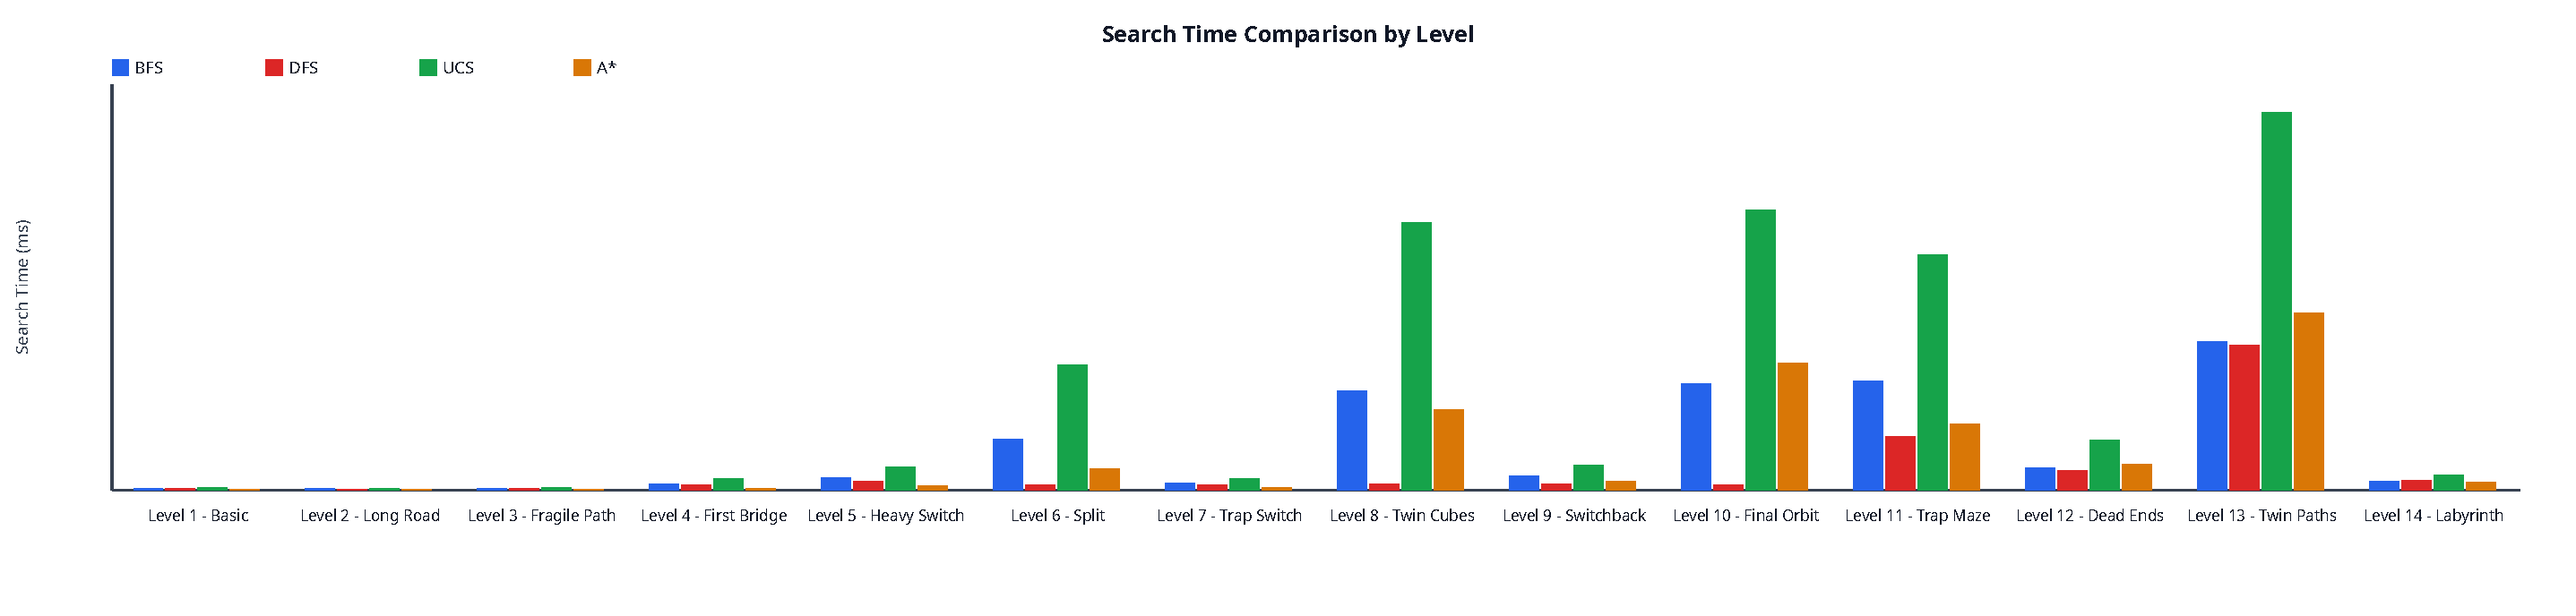
\includegraphics[width=0.92\textwidth]{image/time_comparison.pdf}
\caption{Biểu đồ so sánh thời gian tìm kiếm (\emph{Search Time}) giữa 4 thuật toán.}
\label{fig:time_comparison}
\end{figure}

\begin{figure}[H]
\centering
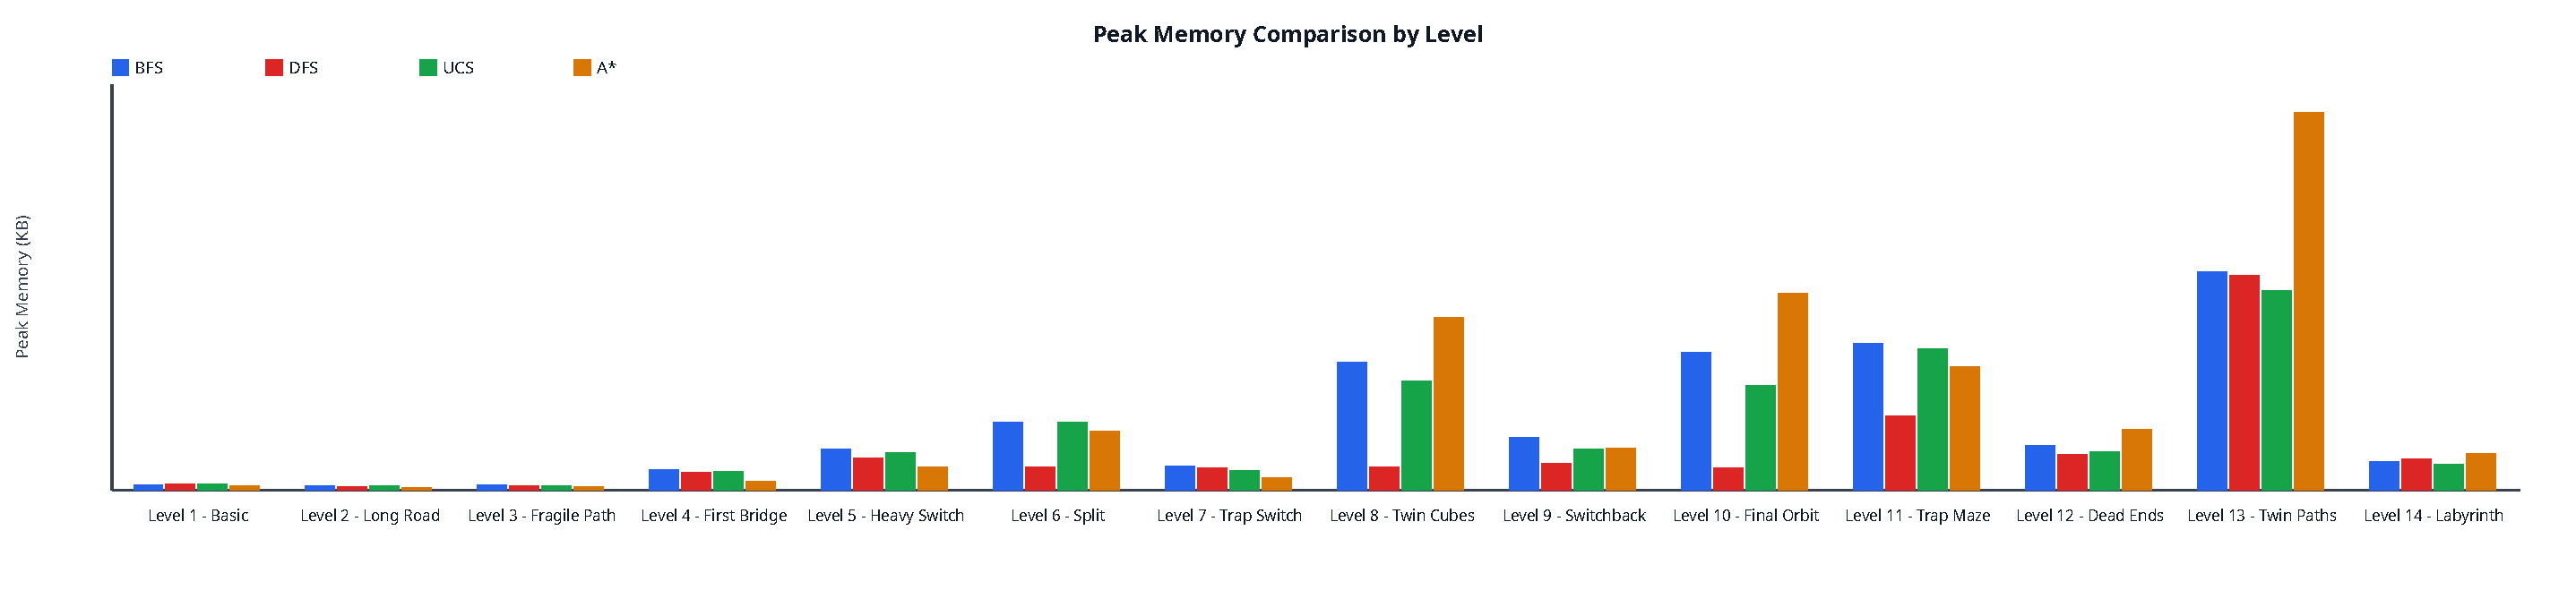
\includegraphics[width=0.92\textwidth]{image/memory_comparison.pdf}
\caption{Biểu đồ so sánh bộ nhớ đỉnh sử dụng (\emph{Peak Memory}) giữa 4 thuật toán.}
\label{fig:memory_comparison}
\end{figure}

\begin{figure}[H]
\centering
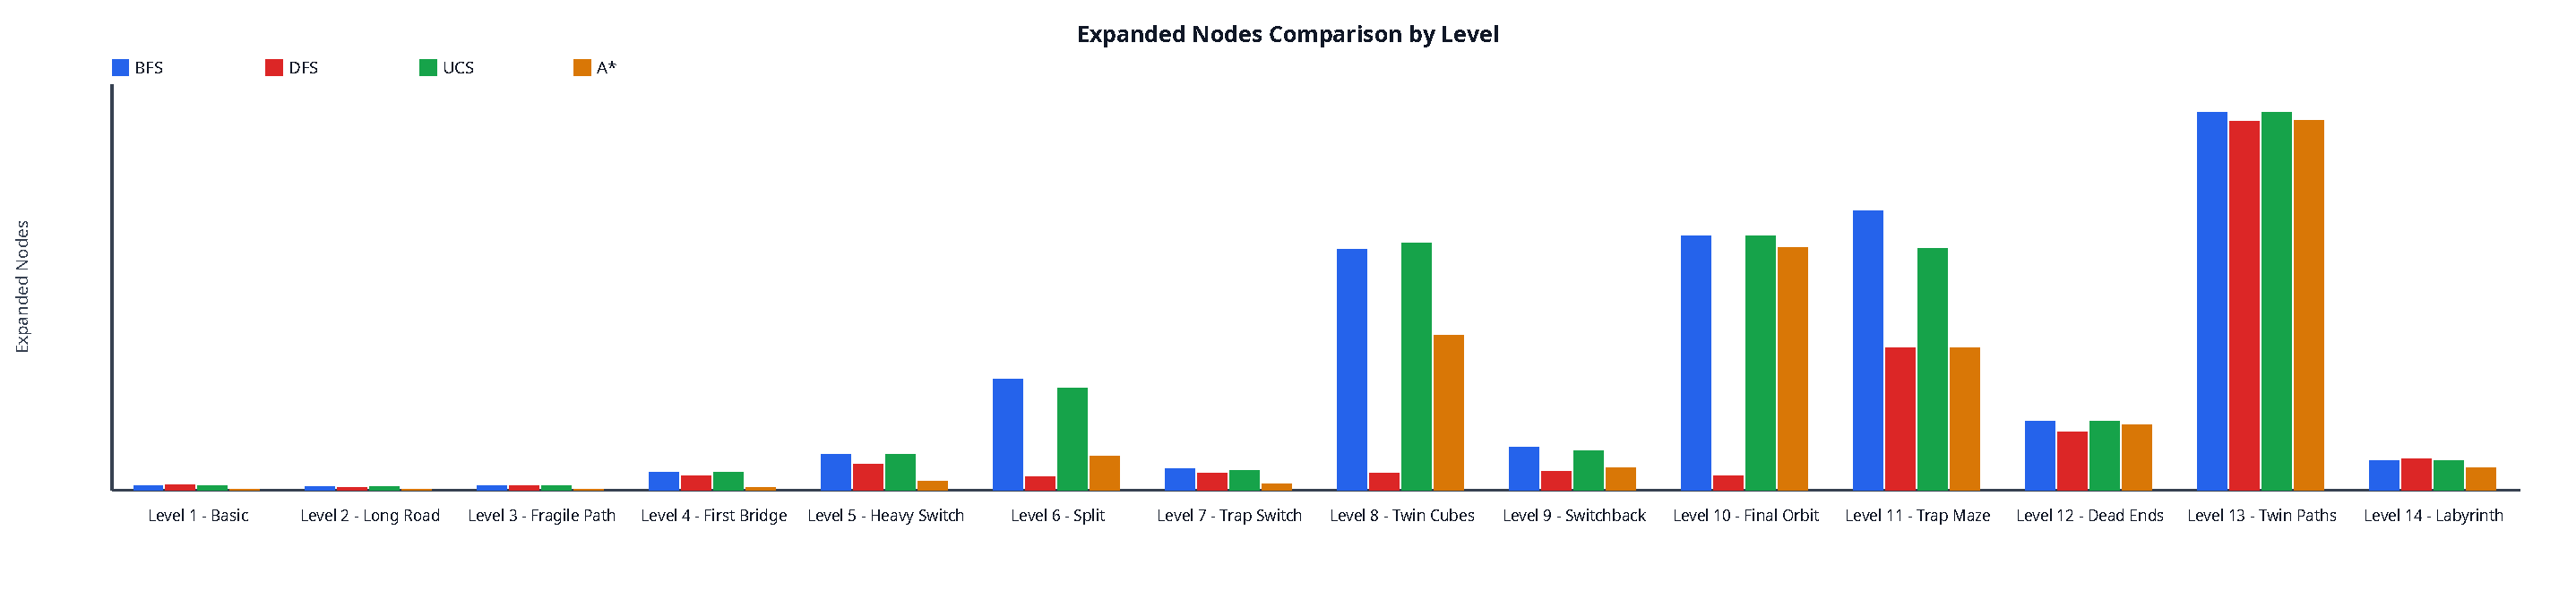
\includegraphics[width=0.92\textwidth]{image/expanded_comparison.pdf}
\caption{Biểu đồ so sánh số nút mở rộng (\emph{Expanded Nodes}) giữa 4 thuật toán.}
\label{fig:expanded_comparison}
\end{figure}

\begin{figure}[H]
\centering
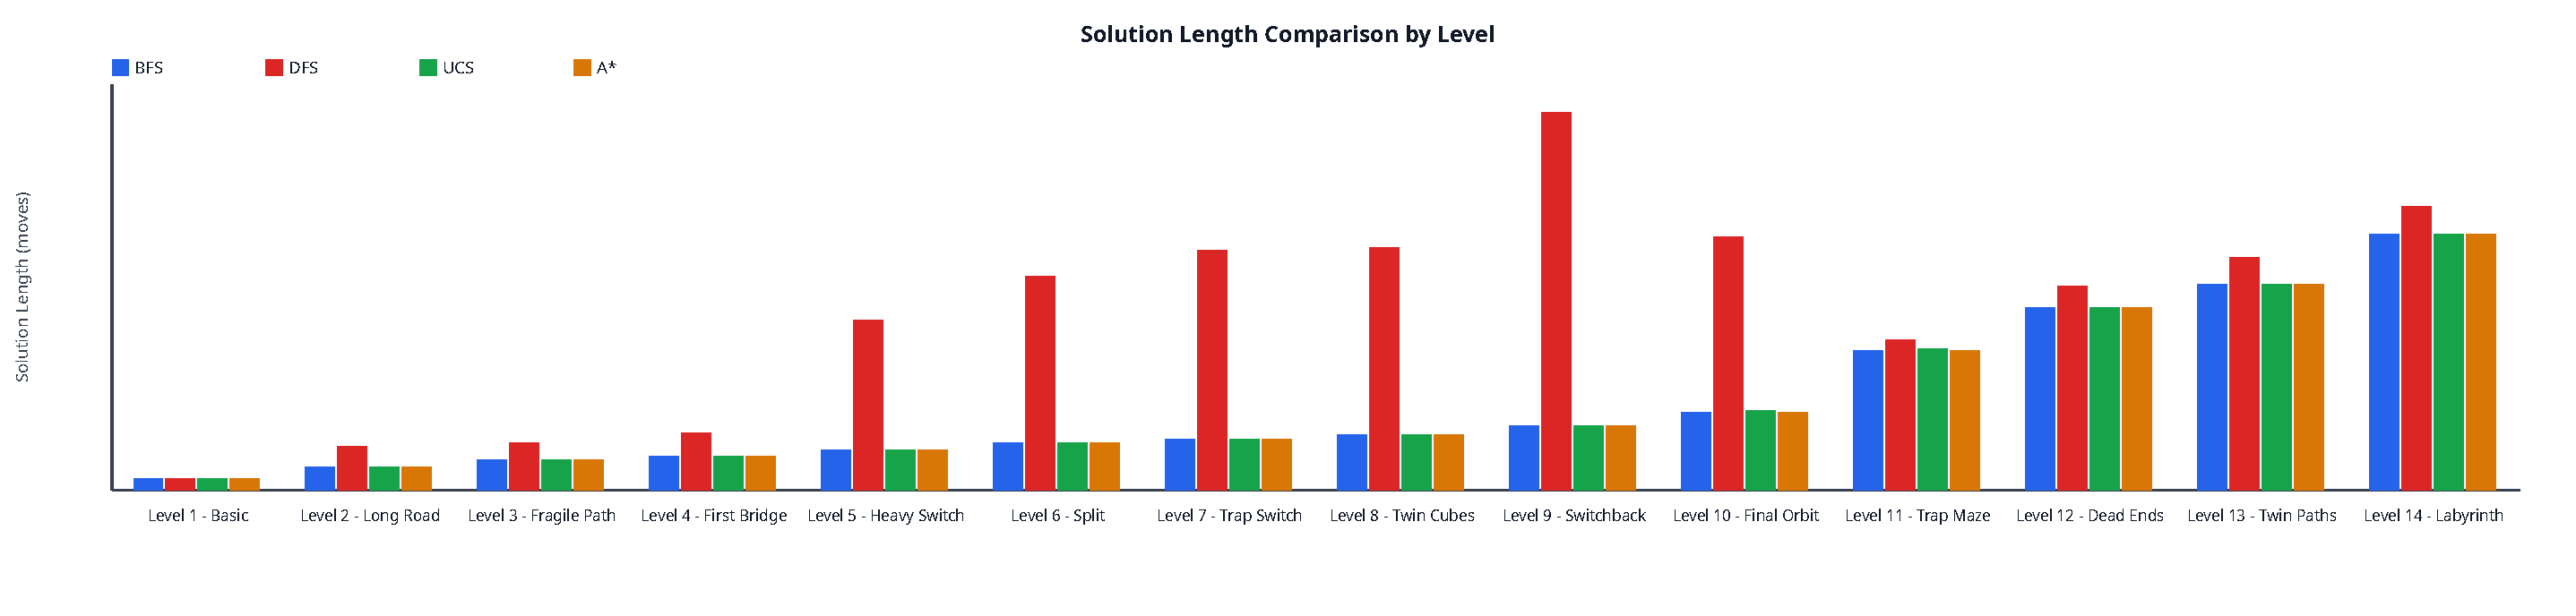
\includegraphics[width=0.92\textwidth]{image/length_comparison.pdf}
\caption{Biểu đồ so sánh độ dài lời giải (\emph{Solution Length}) giữa 4 thuật toán.}
\label{fig:length_comparison}
\end{figure}

\subsection{Nhận xét và Thảo luận}
Từ các bảng số liệu và biểu đồ thực nghiệm trên 14 màn chơi, có thể rút ra những nhận xét chuyên sâu về điểm mạnh, điểm yếu của từng thuật toán như sau:
\begin{enumerate}
    \item \textbf{Thuật toán A* Search:}
    \begin{itemize}
        \item \emph{Ưu điểm:} Luôn tìm được lời giải tối ưu về số bước đi trên toàn bộ 14/14 màn chơi (tương đương BFS). Nhờ hàm Heuristic dựa trên \emph{Reverse 3D BFS} kết hợp khoảng cách Manhattan cho trạng thái phân tách, A* cắt giảm từ \textbf{75\% đến 85\% số nút mở rộng} ở các nhóm \texttt{simple}, \texttt{fragile}, \texttt{switches} (chỉ mở rộng 14--41 nút) và đạt tốc độ nhanh gấp \textbf{2.5--4.3 lần} so với BFS. Ngay cả trên các màn phức tạp như \texttt{Level 6 - Split} và \texttt{Level 11 - Trap Maze}, A* vẫn giảm gần một nửa số nút mở rộng và thời gian chạy so với BFS.
        \item \emph{Nhược điểm:} Ở các màn chơi có nhiều cầu đóng/mở liên tục hoặc đường đi bị ép vào hành lang hẹp dài (\texttt{Level 8}, \texttt{Level 10}, \texttt{Level 13}), khoảng cách hình học trên lưới tĩnh trở nên kém chặt hơn so với ràng buộc trạng thái cầu động, khiến A* tiêu tốn thêm bộ nhớ đỉnh (lên tới $2286.8\text{ KB}$ ở \texttt{Level 13}) để lưu bảng cache Reverse BFS và hàng đợi ưu tiên \texttt{heapq}.
    \end{itemize}
    \item \textbf{Thuật toán Breadth-First Search (BFS):}
    \begin{itemize}
        \item \emph{Ưu điểm:} Đảm bảo tính đầy đủ và luôn tìm được lời giải ngắn nhất theo số bước lăn trên mọi màn chơi. Chi phí thao tác trên mỗi nút rất thấp nhờ hàng đợi \texttt{collections.deque} ($O(1)$).
        \item \emph{Nhược điểm:} Duyệt mù (uninformed) theo từng lớp bán kính nên số nút mở rộng và bộ nhớ tăng nhanh khi không gian trạng thái bùng nổ bởi tổ hợp bitmask của các cầu (\texttt{bridges}) và hai khối tách rời (\texttt{SPLIT}), điển hình ở \texttt{Level 10}, \texttt{Level 11} và \texttt{Level 13} (mở rộng từ $4036$ đến $5996$ nút).
    \end{itemize}
    \item \textbf{Thuật toán Uniform-Cost Search (UCS):}
    \begin{itemize}
        \item \emph{Ưu điểm:} Tối ưu hóa đường đi theo hàm chi phí có trọng số an toàn (phạt khi đè lên ô mỏng \texttt{FRAGILE} và xét trọng số công tắc theo số cầu bị tác động). Đặc biệt ở \texttt{Level 10 - Final Orbit} và \texttt{Level 11 - Trap Maze}, UCS chủ động chọn lộ trình dài hơn 1 bước ($47$ bước thay vì $46$ bước ở Level 10; $84$ bước thay vì $83$ bước ở Level 11) để tránh đi qua các ô mỏng nguy hiểm, đồng thời mở rộng ít nút hơn BFS ở các màn nhiều bẫy (\texttt{Level 6}, \texttt{7}, \texttt{9}, \texttt{11}).
        \item \emph{Nhược điểm:} Thời gian chạy chậm nhất trong 4 thuật toán (trung bình $263.62\text{ ms}$ ở nhóm \texttt{combined}) do chi phí duy trì hàng đợi ưu tiên \texttt{heapq} ($O(\log N)$) kết hợp với việc đánh giá hàm chi phí trạng thái ở mỗi bước sinh nút con.
    \end{itemize}
    \item \textbf{Thuật toán Depth-First Search (DFS):}
    \begin{itemize}
        \item \emph{Ưu điểm:} Trong các màn chơi có không gian trạng thái rộng và nhiều nhánh dẫn về đích (\texttt{Level 6}, \texttt{Level 8}, \texttt{Level 9}, \texttt{Level 10}), DFS đi sâu trực tiếp vào một nhánh hợp lệ nên tìm ra lời giải rất nhanh (chỉ $9.71\text{ ms}$ ở \texttt{Level 10}) với lượng bộ nhớ và số nút mở rộng thấp nhất.
        \item \emph{Nhược điểm:} \textbf{Không đảm bảo tính tối ưu}. Độ dài lời giải trung bình ở nhóm \texttt{combined} lên tới \textbf{140.40 bước}, gấp hơn $2.1$ lần so với mức tối ưu $66.40$ bước của BFS và A* (thậm chí tại \texttt{Level 9 - Switchback}, lời giải của DFS dài $224$ bước so với $38$ bước tối ưu).
    \end{itemize}
\end{enumerate}

\section{Video Demo}
\begin{itemize}
    \item \textbf{Đường dẫn YouTube (Public Link):} \url{https://www.youtube.com/}
    \item \textbf{Nội dung trình diễn trong video:}
    \begin{itemize}
        \item Giới thiệu giao diện đồ họa (GUI), bố cục bàn chơi, các loại ô và các nút điều khiển.
        \item Trình diễn chơi thủ công (lăn khối, kích hoạt công tắc, thắng/thua màn chơi).
        \item Trình diễn chạy các bộ giải tự động (BFS, DFS, UCS, A*) và mô phỏng lại lời giải tìm được trên giao diện.
    \end{itemize}
\end{itemize}

\begin{thebibliography}{9}
\bibitem{russell2020aima}
Stuart Russell and Peter Norvig, \emph{Artificial Intelligence: A Modern Approach}, 4th ed. Pearson, 2020.

\bibitem{bloxorz_coolmath}
Coolmath Games, ``Bloxorz,'' \url{https://www.coolmathgames.com/0-bloxorz}.
\end{thebibliography}

\newpage
\appendix
\section{Phụ lục: Sử dụng công cụ Trí tuệ Nhân tạo Tạo sinh (Generative AI)}
Trình bày cách nhóm sử dụng các mô hình ngôn ngữ lớn (LLMs) trong quá trình thực hiện đồ án (hỗ trợ tìm hiểu tài liệu, kiểm thử, định dạng báo cáo LaTeX) cùng các câu lệnh (prompts) tiêu biểu đã sử dụng.

\end{document}
